\documentclass{article}[12pt]
\usepackage[utf8]{vietnam}
\usepackage{enumerate}
\usepackage{enumitem}
\usepackage{multicol}
\usepackage{listings}
\usepackage[left=2cm,right=2cm,top=2.5cm,bottom=2.5cm]{geometry}
\usepackage{verbatim}
\usepackage{graphbox}
\usepackage{graphicx}
\usepackage{xurl}
\usepackage{fancyhdr}
\usepackage{fancybox,framed}
\linespread{1.3}
\usepackage{lastpage}
\usepackage{floatrow}
\usepackage{floatrow}
\pagenumbering{arabic}
%\pagestyle{fancy}
\newfloatcommand{capbtabbox}{table}[][\FBwidth]

\usepackage[table,xcdraw]{xcolor}
\usepackage{tabularx}
\usepackage{booktabs}

\usepackage{algorithm}
\usepackage{algorithmic}

\usepackage{blindtext}
\usepackage{titlesec}
\usepackage[nottoc]{tocbibind}

\usepackage{hyperref}
\hypersetup{
    colorlinks=true,
    linkcolor=blue,
    urlcolor=blue,
    breaklinks=true,
}

\titleformat*{\section}{\LARGE\bfseries}
\titleformat*{\subsection}{\Large\bfseries}
\titleformat*{\subsubsection}{\large\bfseries}



\begin{document}
    \begin{figure}[h]
        \centering % Căn giữa toàn bộ block này trên trang giấy
        \begin{floatrow}
            % Căn ảnh vào giữa dòng (align=c)
            \ffigbox{
\includegraphics[scale=0.08, align=c]{images/logo.png}}{}
            
            % Căn bảng vào giữa dòng [c]
            \capbtabbox{
                \begin{tabular}[c]{c}
                    \textbf{ĐẠI HỌC KINH TẾ THÀNH PHỐ HỒ CHÍ MINH} \\
                    \textbf{KHOA CÔNG NGHỆ THÔNG TIN KINH DOANH} \\
                    \rule{0pt}{10pt} % Tạo một khoảng không nhỏ phía dưới nếu cần
                \end{tabular}
            }{}
        \end{floatrow}
    \end{figure}
   
    \begin{center}
        
        \textbf{\Large ĐỀ CƯƠNG LUẬN VĂN CAO HỌC} \\ 
    \end{center}
    
    %\vspace{.5cm}
    
    \begin{center}
    %Tên đề tài phải VIẾT HOA
        
        \textbf{\huge Khung phương pháp phân tích sắc thái người dùng Youtube Việt thông qua kiến trúc Transformer.} 
        \\
        
    %Tên đề tài bằng tiếng Anh (nếu có)
    \vspace{.5cm}
        \textit{\textbf{\Large A Transformer-based Framework for Vietnamese YouTube Sentiment Analysis.}}
    \end{center}
    
    \vspace{.5cm}
    
    \Large
    \section{THÔNG TIN CHUNG}
    \begin{itemize}[label = {}]
        
        \item \textbf{Người hướng dẫn:} 
        %Thể hiện dạng: <Chức danh> <Họ và tên> (<Đơn vị công tác>)
        \begin{itemize}
            \item GS.TS. xxx (Bộ môn xxx)
        \end{itemize}{}
    
        
        \item \textbf{Học viên thực hiện:}
        
        %Thể hiện dạng: <Họ và tên sinh viên> (MSSV: )
        \begin{enumerate}
        
            \item xxx (MSHV: yyy) 
        \end{enumerate}

       %Chọn loại thích hợp
        \item \textbf{Loại đề tài:} Nghiên cứu ứng dụng
        
        \item \textbf{Thời gian thực hiện:} Từ \textit{xx/2026} đến \textit{xx/2026}
        
        
    \end{itemize}
    
    \pagebreak 
    
    \section{NỘI DUNG THỰC HIỆN}
    {

    %Mỗi mục dưới đây phải viết ít nhất là 5 câu mô tả/giới thiệu.
    
    \subsection{Giới thiệu về đề tài}
   
    Kể từ khi ra mắt từ năm 2005 và được chính thức bản địa hóa tại Việt Nam vào năm 2014, YouTube, không chỉ dừng lại ở một phương tiện mạng xã hội chia sẻ nội dung số, mà còn đã và đang tạo ra một kho dữ liệu khổng lồ, mang lại giá trị khai thác lớn cho nhiều lĩnh vực. Việc thấu hiểu thái độ và cảm xúc của cộng đồng đối với các nội dung cụ thể không chỉ hỗ trợ đắc lực cho các nhà sáng tạo nội dung mà còn cung cấp nguồn thông tin chiến lược giúp doanh nghiệp đánh giá và định vị thương hiệu. Tuy nhiên, dù thuộc nhóm 20 ngôn ngữ có quy mô cộng đồng sử dụng lớn nhất thế giới \cite{Ethnologue2026}, nhưng việc khai thác dữ liệu này vẫn đối mặt với nhiều thách thức đặc thù. Mà trong đó, sự đa dạng trong văn hóa bản địa vùng miền, kèm với xu hướng giao thoa với văn hóa ngoại quốc, cùng sự bùng nổ của ngôn ngữ mạng (slang), các hệ thống biểu tượng cảm xúc (emoji) và các cấu trúc ngữ pháp biến thể đã tạo ra các rào cản đáng kể đối với các phương pháp phân tích dữ liệu tự động.

    Trong ngữ cảnh khóa luận, đề tài này đề xuất việc xây dựng một khung phương pháp (framework) chuẩn, có thể phân tích sắc thái cảm xúc dựa trên kiến trúc Transformer. Đây là kiến trúc tiên tiến nhất trong xử lý ngôn ngữ tự nhiên (NLP) hiện nay, nổi bật với cơ chế tự chú ý (Self-Attention) cho phép mô hình học máy có thể nắm bắt ngữ cảnh hai chiều một cách hiệu quả \cite{vaswani2017attention}. Nghiên cứu tập trung thiết lập một quy trình hệ thống, từ giai đoạn tiền xử lý dữ liệu đặc thù cho tiếng Việt đến giai đoạn tinh chỉnh (fine-tuning) các mô hình ngôn ngữ tiền huấn luyện (pre-trained models). Kết quả thực nghiệm hướng tới việc tự động hóa quá trình phân loại cảm xúc với độ chính xác cao, đồng thời cung cấp một giải pháp có khả năng tái sử dụng và tùy biến linh hoạt cho nhiều đầu ra khác nhau.

    \subsection{Mục tiêu đề tài}
    
    %Phần này mô tả về động lực để giải quyết vấn đề. 
    Hiện tại, trong kỷ nguyên số, YouTube đã trở thành kênh truyền thông hàng đầu tại Việt Nam. Dẫn chứng bởi Choudhury \cite{choudhury2019five}, Việt Nam là một trong năm thị trường tâm huyết nhất của YouTube trên thế giới. Tính đến cuối năm 2025, theo thống kê của DataReportal \cite{DataReportalVietnam2026}, một nguồn dữ liệu uy tín, YouTube sở hữu một tệp người dùng khổng lồ tại Việt Nam với 62,1 triệu tài khoản, tương đương 61,0\% dân số cả nước. Đồng thời, theo một nguồn thống kê tại Decision Lab \cite{DecisionLab2025Q4}, mức độ thâm nhập của nền tảng cũng lên tới tới 87\% trong quý IV/2025 (hình \ref{fig:decision_lab_iv_2025}), chỉ xếp sau Facebook, Zalo và vượt qua TikTok. Với những con số ấn tượng như vậy, cũng minh chứng rõ nét rằng YouTube đã không chỉ dừng lại là một mạng xã hội phổ biến, mà còn là một hệ sinh thái giàu tiềm năng để khai thác dữ liệu và ứng dụng vào nhiều lĩnh vực đa dạng.
    \begin{figure}[H]
        \centering
        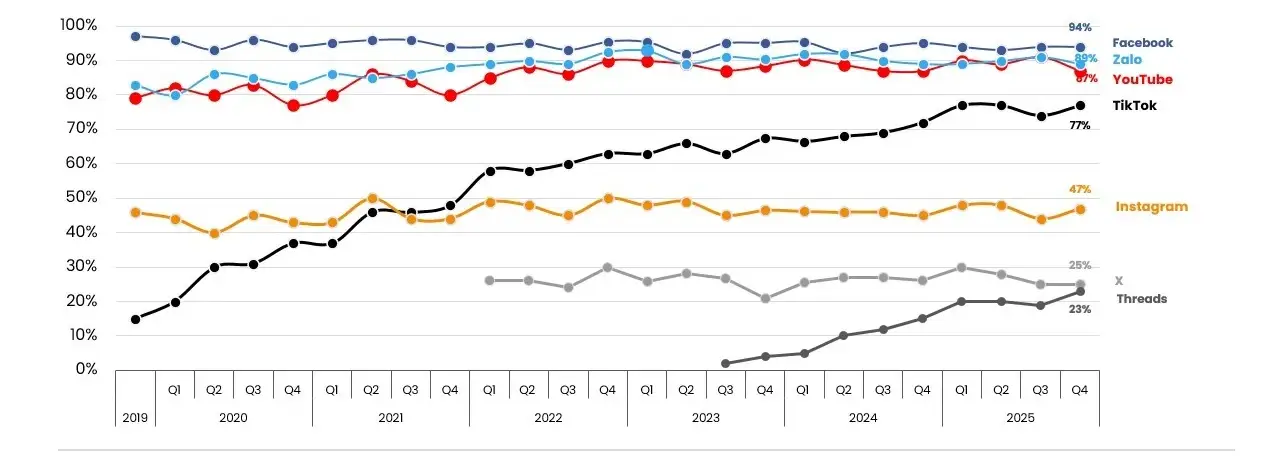
\includegraphics[width=0.9\textwidth]{images/decision_lab_iv_2025_re.png}
        \caption{Biểu đồ tỷ lệ thâm nhập của các nền tảng mạng xã hội dẫn đầu tại Việt Nam, từ Decision Lab, quý IV 2025}
        \label{fig:decision_lab_iv_2025}
    \end{figure}

    Tuy nhiên vì chính sách của nền tảng, nên hoạt động khai thác dữ liệu trên YouTube bị giới hạn trong phạm vi thông tin công khai. Nhưng dẫu vậy, YouTube vẫn là một mạng xã hội kỹ thuật số sở hữu lượng dữ liệu khổng lồ với mức độ tương tác người dùng đặc biệt cao, thể hiện qua hàng triệu lượt bình luận và tương tác trên từng video. Theo triết lý 'Thị trường là những cuộc hội thoại' \cite{levine2009cluetrain}, sự phát triển của Internet đã xóa nhòa rào cản không gian, đặt các tổ chức và thương hiệu trước áp lực phải thấu hiểu hệ sinh thái giao tiếp của khách hàng, tránh việc bị đào thải khỏi cuộc hội thoại chung. Thúc đẩy vấn đề \textbf{lắng nghe mạng xã hội (Social Media Listening)}, nhằm trích xuất các hiểu biết hữu ích và dữ liệu đầu vào có giá trị từ mạng xã hội, càng được chú trọng.
    
    \textbf{Lắng nghe mạng xã hội (Social Media Listening)} được định nghĩa là việc ứng dụng các kỹ thuật khai phá dữ liệu nhằm thực hiện phân tích định lượng, định tính và phân tích ngữ cảnh đối với các chủ đề hoặc từ khóa cụ thể. Quy trình này cho phép theo dõi các dòng chảy hội thoại xung quanh một thực thể cụ thể (như thương hiệu hoặc hashtag), từ đó tổng hợp thông tin để nhận diện cơ hội kinh doanh, tối ưu hóa chiến dịch marketing và nâng cao trải nghiệm khách hàng \cite{ducange2019effective}.
    
    Và trong bối cảnh hiện nay, bên cạnh các dữ liệu mang đặc tính có cấu trúc, thì với sự phát triển đột phá của học máy (Machine Learning) đã mở ra khả năng khai thác sâu sắc các nguồn dữ liệu phi cấu trúc, đặc biệt là văn bản. Vốn là nguồn dữ liệu quan trọng chứa đựng các trạng thái nội tâm (private states), như ý kiến ý kiến, niềm tin, suy nghĩ, tình cảm, cảm xúc, mục tiêu, đánh giá và phán đoán của con người \cite{wiebe2005annotating}. Hệ quả tất yếu là sự kết hợp với bài toán đánh giá tính phân cực cảm xúc trong văn bản, hay còn gọi là \textbf{Phân tích sắc thái cảm xúc (Sentiment Analysis - SA)} nhằm bổ sung khai thác dữ liệu mạng xã hội.

    Như đã đề cập, dữ liệu công khai trên nền tảng YouTube rất phong phú với sự đa dạng về lĩnh vực, hình thành nên một kho dữ liệu đa miền (multi-domain) khổng lồ. Trong khi bài toán phân tích sắc thái cảm xúc ở các ngôn ngữ phổ biến đã đạt được nhiều thành tựu đáng kể (\cite{shen2025zero}, \cite{zhao2024multi}, \cite{lee2026dimabsa}, \cite{zhao2025interpretable}, \cite{guo2024mvindemo}), các nghiên cứu đối với tiếng Việt hiện nay phần lớn vẫn chỉ tập trung vào các tập dữ liệu ngách thuộc một miền cụ thể (\cite{nguyen2025like}, \cite{minh2024fine}, \cite{le2025hybrid}).

    Bên cạnh đó, dù nằm trong top 20 ngôn ngữ có lượng người dùng lớn nhất \cite{Ethnologue2026}, tiếng Việt vẫn đối mặt với những thách thức đặc thù. Sự khác biệt về phương ngữ và từ địa phương tạo ra rào căn không nhỏ cho việc xử lý ngôn ngữ tự nhiên. Đồng thời, sự hội nhập văn hóa sâu rộng đã thúc đẩy hiện tượng trộn mã (code-switching) (ví dụ: "sản phẩm nhìn rất chill") trở nên phổ biến và biến đổi không ngừng theo thời gian. Sự thay đổi trong cách diễn đạt cảm xúc cùng vốn từ vựng mới đòi hỏi các mô hình học máy phải có tính thích nghi cao (adaptability) để tránh hiện tượng lỗi thời trước những biến động ngôn ngữ xã hội.

    Đồng thời, khi xét đến phương diện ngôn ngữ học, tiếng Việt có hơn một nửa vốn từ là Hán - Việt \cite{phanngoc2000}. Những từ ngữ này đều mang một sắc thái ngữ nghĩa (hay tu từ) khiến cho nó khác biệt rõ rệt so với các từ thuần Việt đồng nghĩa \cite{cao2003tiengviet}. Ngoài ra, việc sử dụng chữ Quốc ngữ cũng triệt tiêu đi khả năng phân biệt thị giác giữa các từ đồng âm khác nghĩa \cite{cao2003tiengviet}. Điều này khiến các mô hình học máy gặp phải khó khăn trong việc bóc tách các sắc thái biểu cảm vốn ẩn chứa trong tầng nghĩa từ nguyên, đặc biệt khi ngữ cảnh bình luận trên YouTube thường ngắn, rời rạc và chứa nhiều thông tin nhiễu.
    
    Và một bài toán nan giải khác nằm ở sự khác biệt trong hành vi người dùng giữa hai dạng tương tác \textbf{tĩnh (VOD - Video on Demand)} và \textbf{động (Livestream)} \cite{huo2025live}. Với tương tác tĩnh, người dùng có thời gian suy ngẫm và trau chuốt nội dung bình luận. Ngược lại, tương tác trong livestream (Live Chat) đòi hỏi sự phản hồi tức thì, ngắn gọn và mang tính bộc phát. Hệ quả là các mô hình truyền thống thường bị giảm độ chính xác hoặc mất đi khả năng xử lý do độ nhiễu cực cao và sự không nhất quán về mặt cấu trúc câu trong dữ liệu thời gian thực.
    
    Cuối cùng, với những dữ liệu có độ dài, người dùng thường có xu hướng lồng ghép nhiều luồng cảm xúc trái ngược (ví dụ như "giọng hay nhưng nội dung tệ"). Và nếu chúng ta chỉ dừng lại ở việc phân loại đơn giản "tích cực" hoặc "tiêu cực", thì mô hình sẽ làm mất đi các giá trị thông tin cốt lõi. Điều này đòi hỏi bài toán phân tích sắc thái cảm xúc ban đầu trở thành Phân tích cảm xúc dựa trên khía cạnh (Aspect-Based Sentiment Analysis - ABSA) để bóc tách chính xác thái độ của người dùng đối với từng thuộc tính cụ thể của đối tượng.

    Với những vấn đề trên, đặt ra một vấn đề thực tiễn hết sức cấp thiết, đó là làm thế nào để xây dựng một khung phương pháp (framework) chuẩn, có thể phân tích sắc thái cảm xúc dựa trên kiến trúc Transformer, nhằm giải quyết các thách thức đặc thù của dữ liệu YouTube Việt Nam. Đây không chỉ là một bài toán học thuật mà còn mang tính ứng dụng cao, khi kết quả có thể hỗ trợ đắc lực cho các nhà sáng tạo nội dung và doanh nghiệp trong việc thấu hiểu cộng đồng người dùng, từ đó đưa ra các chiến lược phát triển nội dung và kinh doanh hiệu quả hơn.

    \subsection{Phạm vi của đề tài}
    
    \subsubsection{Phân tích sắc thái cảm xúc (Sentiment Analysis - SA)}

    \textbf{Phân tích sắc thái cảm xúc}, hay còn gọi là khai thác ý kiến (Opinion mining), được định nghĩa là lĩnh vực nghiên cứu các quan điểm, thái độ và cảm xúc của con người được diễn đạt thông qua văn bản. Về mặt kỹ thuật, quá trình này liên quan đến việc trích xuất và phân loại các thông tin mang tính chủ quan nhằm xác định thái độ của người viết đối với một thực thể cụ thể \cite{liu2010sentiment}.
    Thông thường, thuật ngữ \textit{đối tượng} ($o$) được dùng để chỉ thực thể mục tiêu mà người viết hướng tới, chẳng hạn như sản phẩm, dịch vụ, cá nhân hoặc tổ chức. Về mặt cấu trúc, một đối tượng $o$ có thể được phân tách thành một hệ thống phân cấp bao gồm các thành phần ($T$) và các thuộc tính ($A$).
    
    \textit{Ví dụ:} Nếu xét đối tượng $o$ là một "Video", các thành phần $T$ có thể bao gồm "nội dung", "âm thanh", "diễn viên"; các thuộc tính $A$ tương ứng có thể là "độ chân thực" hay "kỹ năng diễn xuất". Và trong đó, thành phần "nội dung" lại có thể được chia ra với các thành phần con $T_1$ như "phân cảnh", "thông điệp truyền tải", "lời thoại",... và các thuộc tính con $A_1$ như "độ hấp dẫn", "độ sâu sắc", "tính logic",...
    
    Dựa trên định nghĩa này, đối tượng $o$ có thể được biểu diễn dưới dạng một cấu trúc cây phân cấp $o: (T, A)$, trong đó gốc là chính đối tượng $o$, các nút nội bộ là các thành phần và các lá đại diện cho các thuộc tính chi tiết. Mặc dù cảm xúc có thể được biểu đạt tại bất kỳ nút nào trên cây, nhưng việc khai thác trực tiếp trên cấu trúc này thường gặp khó khăn do độ phức tạp về mặt tính toán và xử lý ngôn ngữ tự nhiên.
    
    Do vậy, để tối ưu hóa quá trình khai thác, cấu trúc cây thường được đơn giản hóa bằng phương pháp "làm phẳng" (flattening). Khi đó, tất cả các thành phần và thuộc tính được đại diện bằng thuật ngữ \textbf{khía cạnh} (aspect) hoặc \textbf{đặc tính} (feature), ký hiệu là $f$. Và một cảm xúc trực tiếp lúc này được mô hình hóa bằng một \textit{bộ 5 thành phần (quintuple)}, $(o, f, so, h, t)$. Trong đó, $so$ là hướng cảm xúc (sentiment orientation) (ví dụ như tích cực, tiêu cực hoặc trung tính); $h$ là chủ thể diễn đạt cảm xúc (holder); và $t$ là thời điểm cảm xúc được biểu đạt.
    
    Đối với một văn bản $d = \langle s_1, s_2, \dots, s_m \rangle$, trong đó $s_i$ là các câu cấu thành, mục tiêu của việc phân tích cảm xúc được phân định rõ ràng qua ba cấp độ nghiên cứu chính:
    \begin{itemize}
        \item \textbf{Cấp độ văn bản (Document-level):} Xác định hướng cảm xúc tổng thể của toàn bộ văn bản $d$ đối với đối tượng $o$, thường được biểu diễn bằng cặp $(o, so)$.
        \item \textbf{Cấp độ câu (Sentence-level):} Xác định cảm xúc của từng câu $s_i$ đối với đối tượng $o$. Cấp độ này thường đi kèm với nhiệm vụ phân loại tính chủ quan (subjectivity classification) để phân tách câu chứa ý kiến và câu nêu sự thật.
        \item \textbf{Cấp độ khía cạnh (Aspect-level):} Xác định hướng cảm xúc đối với từng khía cạnh cụ thể $f_j$ của đối tượng $o$ được đề cập trong câu $s_i$, biểu diễn bằng bộ $(s_i, f_j, so)$. Đây là cấp độ chi tiết nhất, cho phép xử lý các văn bản chứa nhiều ý kiến phức tạp và trái ngược nhau.
    \end{itemize}

    \subsubsection{Khung phương pháp (Framework)}
    
    - Transformer-based models ?
    - Vietnamese YouTube data ?
    - Framework hoạt động?

    \subsection{Cách tiếp cận dự kiến}
    Để giải quyết bài toán phân tích sắc thái cảm xúc trên dữ liệu YouTube Việt Nam, đề tài sẽ áp dụng một cách tiếp cận dự kiến bao gồm các bước chính sau đây:
    - Từng bước pipeline ở đây

    \subsection{Kết quả dự kiến của đề tài}
    Trong phạm vi khóa luận, các kết quả dự kiến có thể đạt được được trình bày như sau:
    \begin{itemize}
        \item Hoàn thiện được một hình mẫu (framework) hậu diễn giải cho mô hình Meta-Learning cụ thể là các phương pháp dựa trên Gradient-based thông qua các phương pháp hậu diễn giải.
    \end{itemize}
    
    
    \subsection{Kế hoạch thực hiện}
    Đề tài nghiên cứu luận văn cao học được thực hiện tại Khoa Công nghệ thông tin Kinh doanh, trường Đại học Kinh tế TPHCM.
    
    Thời gian thực hiện đề tài nghiên cứu 06 tháng kể từ tháng xx/2026 đến xx/2026. Kế hoạch thực hiện chi tiết cho đề tài nghiên cứu được liệt kê như trong bảng \ref{tab:kehoach}.

    \begin{table}[htbp]
        \centering
        \renewcommand{\arraystretch}{1.4}
        \begin{tabularx}{\textwidth}{|>{\raggedright\arraybackslash}X|c|}
        \hline
        \rowcolor[gray]{0.9}
        \textbf{Công việc} & \textbf{Thời gian thực hiện} \\ \hline
        Tìm hiểu các hướng tiếp cận và công trình liên quan & 01/01/2026 - 15/02/2026 \\ \hline
        Khảo sát, đánh giá các công trình tiêu biểu và hoàn thiện đề cương & 16/02/2026 - 16/03/2026 \\ \hline
        Nghiên cứu các phương pháp giải quyết bài toán diễn giải cho Meta-Learning & 17/03/2026 - 20/04/2026 \\ \hline
        Đề xuất phương pháp cải tiến, thực nghiệm và báo cáo giữa kỳ & 21/04/2026 - 06/05/2026 \\ \hline
        Thực hiện thực nghiệm bổ sung, đánh giá kết quả và viết bản thảo luận văn & 07/05/2026 - 30/06/2026 \\ \hline
        Hoàn thiện quyển luận văn, chỉnh sửa theo góp ý của GVHD và chuẩn bị bảo vệ & 01/07/2026 - 15/07/2026 \\ \hline
        \end{tabularx}
        \caption{Bảng kế hoạch thực hiện đề tài khóa luận}
        \label{tab:kehoach}
    \end{table}
    
    }
    \pagebreak 

    %TÀI LIỆU TRÍCH DẪN
    \bibliographystyle{ieeetr}
    \bibliography{ref}
    \nocite{*}

%    \pagebreak
    %\begin{table}[h]
    %\centering
        %\begin{tabular}{p{7cm}p{7cm}}
        %\textbf{\begin{tabular}[c]{@{}c@{}}\\XÁC NHẬN\\CỦA NGƯỜI HƯỚNG DẪN\\ \textit{(Ký và ghi rõ họ tên)}\end{tabular}} & \textbf{\begin{tabular}[c]{@{}c@{}}\textit{TP. Hồ Chí Minh, ngày 16 tháng 03 năm 2026}\\NHÓM SINH VIÊN THỰC HIỆN\\\textit{(Ký và ghi rõ họ tên}) \end{tabular}}
        %\end{tabular}
    %\end{table}
    
\end{document}


